\section{Satellite Galaxies Around a Massive Central}

In this section we will investigate the spherical distribution of satellite galaxies around a massive central galaxies, and attempt to  fit a function to simulated data. Their density distribution $n$ can be described as

\begin{equation}
    n(x) = A\left<N_{sat}\right>\left(\frac{x}{b}\right)^{a-3}\exp{\left[-\left(\frac{x}{b}\right)^{c}\right]}\label{eq:nx}
\end{equation}

Here $x$ is the radius relative to the virial radius, i.e. $x \equiv r/r_{vir}$ with $x < x_{max} = 5$. $a$, $b$ and $c$ are free parameters, $\left<N_{sat}\right>$ is the mean number of satellites per halo and $A = A(a,b,c)$ normalizes this profile such that $\int\int\int_V n(x)dV = \left<N_{sat}\right>$. In this work we will mainly look at tt the number of satellites in the infinitesimal range $\left[x, x+dx\right>$. This is given by

\begin{equation}
    N(x)dx = n(x)4\pi x^2dx\label{eq:Nx}
\end{equation}

\lstinputlisting[caption={Satellite galaxy distribution code}, linerange={7-17}]{fitting.py}

\subsection{Maximization}\label{sec:maxi}

We start by searching for the maximum of the distribution given by equation \ref{eq:Nx}, for this we will assume $a=2.4$, $b=0.25$, $c=1.6$. $x_{max}=5$, $\left<N_{sat}\right>=100$ and $A=256/(5\pi^{3/2})$. Instead of searching for the maximum, we instead search for the minimum of $-N(x)dx$ which gives the equivalent resulting $x$. Visually inspecting the distribution (Figure \ref{fig:maximum}), we see a clear peak at $x \sim 0.5$. To be safe we set the edges of our initial bracket at $x_{min} = 0$ and $x_{max} = 5$ and then apply a bracketing algorithm to find a three-point bracket around the minimum. Then we use this bracket as input to the golden section search algorithm to find the $x$-value at the peak. We find the following brackets and minimization results:  

\lstinputlisting[caption={Results of the maximization algorithm.}]{results/maxi_results.txt}

We also show the distribution and the exact location of this peak in Figure \ref{fig:maximum}. We can see that the algorithms have perfectly discovered the maximium of this distribution.

\begin{figure}
    \centering
    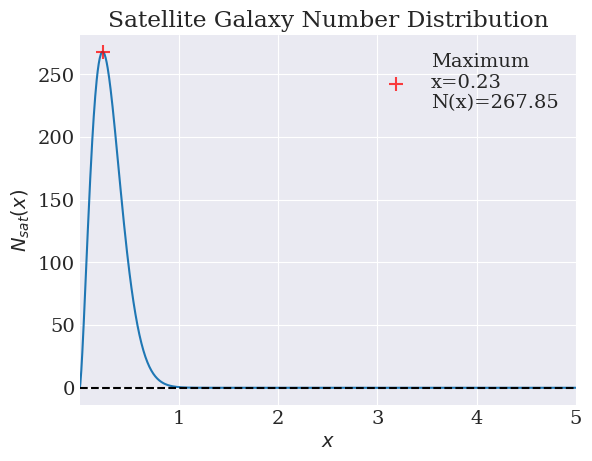
\includegraphics[width=0.8\textwidth]{results/maxi.png}
    \caption{Distribution of the number of galaxies in the infinitesimal range $\left[x, x+dx\right>$ described by equation \ref{eq:Nx}. The red cross indicates the position of the maximum of this distribution discovered using the golden search algorihtm as described in Section \ref{sec:maxi}}
    \label{fig:maximum}
\end{figure}

\lstinputlisting[caption={Code calling the maximization algorithm}, linerange={26-64}]{galaxies.py}
\lstinputlisting[caption={Code for the maximization algorithm}, linerange={199-287}]{ancillary.py}

\subsection{Data Fitting}\label{sec:datafitting}

We import the five datafiles provided for this hand-in which contain satellite galaxies for halos in increasing mass bins ranging from $10^{11} M_{\odot}$ up to $10^{15} M_{\odot}$. Each file contains a number of halos, $N_{halo}$, and the distances of each satellite galaxy from its center massive galaxy. For each dataset we can immediately compute $\left<N_{sat}\right>$ by dividing the total number of satellite galaxies by $N_{halo}$. We bin the data in 20 bins from $x = 10^{-4}$ to $x=5$ in log-space. We set the lower limit above $x=0$ for computational reasons because equation \ref{eq:Nx} is not defined there. We opt to show the distributions in log-space to better visualize the low $x$ region. The decision for 20 bins is relatively arbitrary but appears to result in plots that are easily interpretable. We show the binned data together with $N_{halo}$ for each dataset in Figure \ref{fig:sat_data}.

\begin{figure}
    \centering
    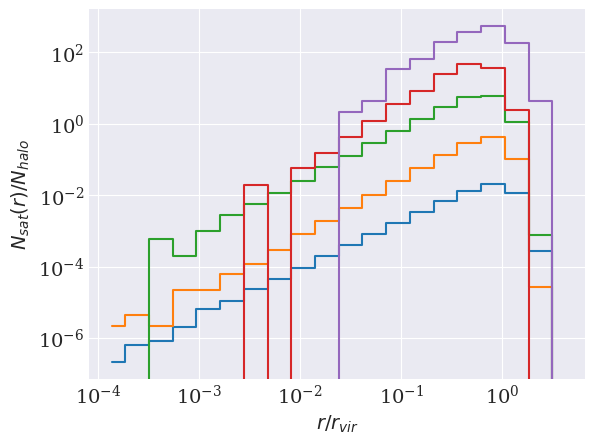
\includegraphics[width=\textwidth]{results/satellite_data.png}
    \caption{Binned satellite galaxy distance data divided into five mass bins of their massive galaxy halo as indicated on the right. The total number of halos over which the satellite galaxies are distributed is also indicated on the right.}
    \label{fig:sat_data}
\end{figure}

In the next two subsections we will first describe our two approaches to fit equation \ref{eq:Nx} to these distributions. In Section \ref{sec:fitresults} we present the results of our fitting algorithms applied to the data, combined with a brief statistical analysis.

\lstinputlisting[caption={Code to import data, and make the plot of Figure \ref{fig:sat_data}}, linerange={9-23, 67-97}]{galaxies.py}
\lstinputlisting[caption={Code that calls the fitting procedures and performs the statistical tests}, linerange={100-194}]{galaxies.py}

\subsubsection{Chi-Squared}

These data are discrete counts, so therefore they should be fit by a Poisson distribution. However we start with an 'easy' $\chi^2$ fit with Poisson variance (i.e. $\sigma^2 = \mu$) to compare to the proper unbiased fit. This means that we want to minimize the function

\begin{equation}
    \chi^2 = \frac{\left(y_i - \mu(x_i | \boldsymbol{p})\right)}{\mu(x_i | \boldsymbol{p})}.\label{eq:chi2}
\end{equation}

Where $x_i$ and $y_i$ are the bin center and bin counts respectively. $\mu$ is a function of the parameter describing the expected value in any particular bin, which is given by

\begin{equation}
    \mu\left(x_i | \boldsymbol{p})\right) = \tilde N_i = \int_{x_i}^{x_{i+1}} N(x)dx.\label{eq:mean}
\end{equation}

We minimize Equation \ref{eq:chi2} for each dataset separately using the Levenberg-Marquardt algorithm. As a good starting guess we use the same parameters as in Section \ref{sec:maxi}, i.e. $a=2.4$, $b=0.25$, $c=1.6$. Another important thing to note is that the normalization constant $A$ is a function of these three parameters which keep changing. We therefore compute a new value for $A$ each time the parameters are shift by first integrating over $N(x)$ from $x_{min}=10^{-4}$ to $x_{max}=5$ using Romberg integration and $A=1$. We then compute $A$ by dividing $\left<N_{sat}\right>$ by the result of this integral.

\lstinputlisting[caption={Code for the chi-squared fitting computing $\tilde N_i$ and calling the Levenberg-Marquardt algorithm}, linerange={20-53}]{fitting.py}
\lstinputlisting[caption={Code for the Marquardt-Levenberg algorithm}, firstline={4}]{lm_method.py}

\subsubsection{Poisson}

For the Poisson fit we have two options: we can either use the same binned data as is used for the $\chi^2$ fit, or we can opt to not use bins at all. In this latter case we pretend as though we did bin the data, however with bin size sufficiently small such that each bin contains either 0 or 1 objects. Doing this allows us to make better use of the data at the cost of more computational load. In the worst case, namely the first dataset, this difference is a factor on the order of $10^4$. Unfortunately while implemented, we have been unable to use this binless fitting as computing time exceeds the maximum alloted time of ten minutes. Therefore we opt to fit the data here using the same bins as in the previous section. The log-likelihood of a Poisson distribution is given as

\begin{equation}
    -\ln \mathcal{L}(\boldsymbol{p}) = -\sum_{i=0}^{N-1} \left(y_i\ln\left[\mu(x_i | \boldsymbol{p}))\right] - \mu(x_i | \boldsymbol{p})) - \ln(y_i!)\right).\label{eq:logL}
\end{equation}

When minimizing this equation we can ignore the last term, $\ln(y_i!)$ because it is independent of the parameters we are fitting and therefore constant. We are then left with only the first two terms in the sum. For the minimization we will make use of the downhill simplex method where we initialize one of the vertices of the first simplex using the same parameters as before ($a=2.4$, $b=0.25$, $c=1.6$). We initialize the other three vertices by adding one to parameter $i$ for vertex $i$.

We also attempted to implement the Quasi-Newton method to minimize the log likelihood function, however this also has proven unsuccesful due to extremely steep gradients which often led the line minimization algorithm to regions in parameter space where the likelihood function is not defined. This only led to NaN values as a result for the parameters. While not used, the code is still included at the end of this report.

\lstinputlisting[caption={Code to compute the Poisson likelihood, and to call the minimization functions}, firstline={56}]{fitting.py}
\lstinputlisting[caption={Downhill simplex code}, linerange={290-377}]{ancillary.py}

\subsection{Fit Results}\label{sec:fitresults}

We apply the fitting methods described in the previous sections to each of the datasets \texttt{satgals\_m1i.txt} with $i \in [1,5]$, and present the results in Figure \ref{fig:fitres}. We also include the parameters and $\chi^2$ or $\ln\mathcal{L}$ values in Table \ref{tab:fit_vals}

\begin{figure}
    \centering
    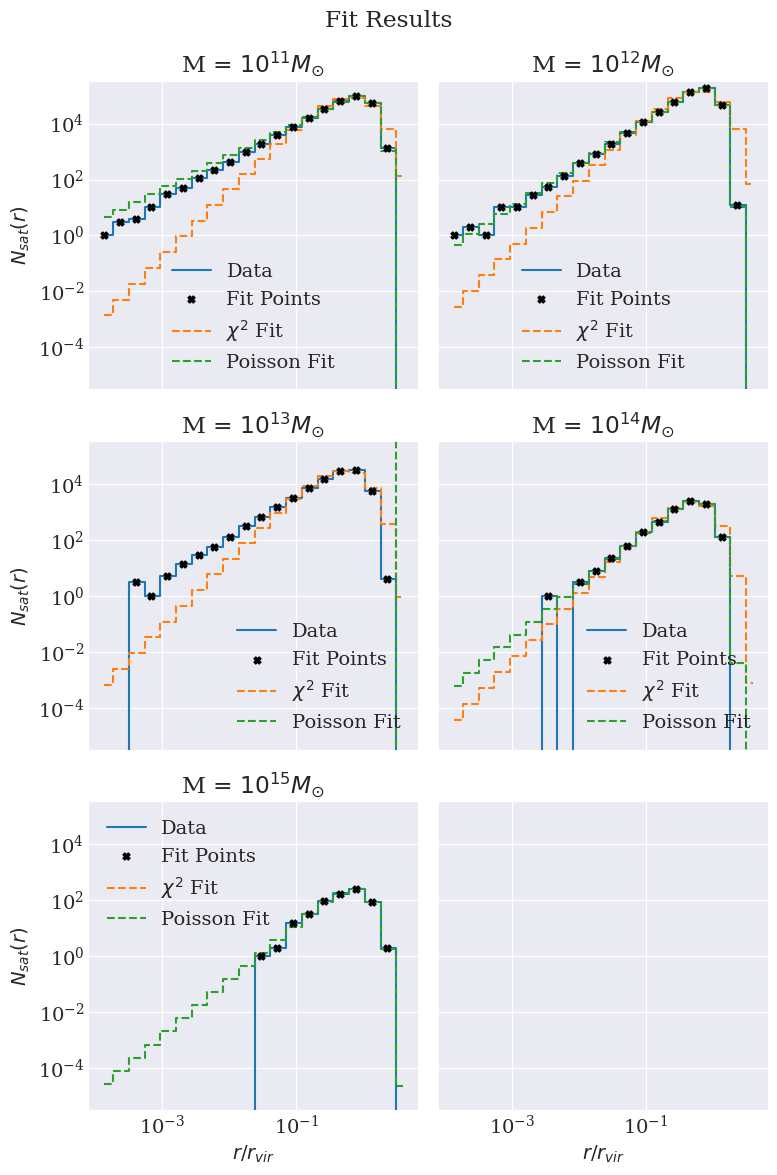
\includegraphics[width=\textwidth]{results/fitresults.png}
    \caption{}
    \label{fig:fitres}
\end{figure}

\begin{table}[h]
    \centering
    \begin{tabular}{|c|c|c|c|c|c|c|}
    \hline
    $M$ & $\left<N_{sat}\right>$ & $a$ & $b$ & $c$ & $\chi^2$ & $\ln\mathcal{L}$   \\
    \hline
    \input{results/fitresults.txt} \\
    \hline
    \end{tabular}
    
    \caption{Numerical results of both fitting procedures. For each of the five datasets we first present the resutls of the $\chi^2$ fit, and the the results of the Poisson fit, this is clearly visible through which field out of $\chi^2$ or $\ln\mathcal{L}$ is filled in. The values provided here are rounded to only 2 significant digits to let them fit on the page. However the full values are given at the end of this report.}
    \label{tab:fit_vals}
\end{table}

In the figure we can see that the $\chi^2$ fits appear to have performed quite badly for all datasets, underestimating the amount of satellite galaxies at low $x$ and exteremely overestimating this in the highest $x$ bin in the first three datasets. In the last two sets this pattern appears reversed and the peaks of the data- and model distributions do not match anymore. This is possibly caused by the fact that there is almost no data below $x \sim 10^{-2}$ which confuses the $\chi^2$ statistic. The Poisson fits on the other hand appear to fit quite well to the data. In most of the plots the Poisson fit appears to at most be off by a few from the real data which could just be due to noise. Only in the $10^{11} M_{\odot}$ fit can we see that the Poisson fit appears to be biased towards higher values in the low $x$ end, and appears to be 'off' by a few hundred to a thousand in the highest $x$ bin. 



But to draw some quantitative conclusions about these fits we have to perform some statistical test. We will do a G-test on the binned fit results and binned data. This G statistic is defined as

\begin{equation}
    G = 2~\sum_i^N O_i\ln\left(\frac{O_i}{E_i}\right)\label{eq:G}.
\end{equation}

Where $O_i$ is the observed number of instances in a bin, which should always be an integer, and $E_i$ is the expected number of observations in a bin. This latter value is the expected model value in a given bin, and therefore is not limited to being an integer. We can use this G statistic in a goodness of fit test for $\chi^2$ to compute the Q-value, which is equivalent to the p-value. This Q is defined as

\begin{equation}
    Q = 1 - \frac{\gamma\left(\frac{k}{2},\frac{x}{2}\right)}{\Gamma\left(\frac{k}{2}\right)}\label{eq:Q}
\end{equation}

With 

\begin{align}
    \gamma(s, x) &= \int_0^x t^{s-1}e^-t dt \\
    \Gamma(z) &= \int_0^{\infty} t^{z-1}e^{-t}dt
\end{align}

the lower incomplete gamma function, and the gamma function respectively which we compute using \texttt{scipy.special.gammainc} and \texttt{scipy.special.gamma}. $k$ is the number of degrees of freedom in the data, which is given by $N - M$ where $N$ is the number of data points and $M$ is the number of free parameters. In our case $N$ is the number of data bins which we have set to $20$, and $M$ is the number of parameters we fit, 3, but also $\left<N_{sat}\right>$ which sets the area under the curve. This means $M=4$ and therefore the total number of degrees of freedom $k = 16$. We compute the G and Q values for each fit on each dataset, and present the results in Table \ref{tab:stats}.\footnote{The code for this section was already given in Section \ref{sec:datafitting} because it is done in the same loop as all the fitting procedures.}

\begin{table}[h]
    \centering
    \begin{tabular}{|c|c|c|c|}
    \hline
    $M$ & Method & $G$ & $Q$ \\
    \hline
    \input{results/stats.txt} \\
    \hline
    \end{tabular}
    \caption{G-test values for each dataset and each fitting method.}
    \label{tab:stats}
\end{table}

A Q value lower than $\sim~0.1$ would indicate that our fit is bad. Unfortunately, this appears to be the case for all of the fits computed in this report. Most of the Q-values reported here take on the exact same value, which is an indication that our G values are extremely high and therefore also statistically extremely bad fits. We see one negative value in the G value for one of the Poisson fits, this in principle should never happen. Especially not a negative number that is as large as this is. This is another strong indication that there is most likely something wrong with the fit for that particular dataset. 

The only thing one might be able to conclude from these statistics is the fact that, while the fits look reasonably good when inspected visually, when analyzing them quantiatively, with the G-statistic, they are actually quite bad. Although it is also important to note here that another statistic might have yielded better, or at least different, results than what is presented here.

\lstinputlisting[caption={Unrounded numerical values for the fitting parameters presented in Table \ref{tab:fit_vals}.}]{results/full_fitresults.txt}
\newpage
\lstinputlisting[caption={Code for the Quasi-Newton algorithm which was too prone to divergence and is therefore sadly unused in this report}, firstline={380}]{ancillary.py}

